\section{Applications des suites}

\subsection{Placements}

\subsection{Emprunts}

\subsubsection{Emprunts à amortissements constants}

\subsubsection{Emprunts à versements constants}

\subsection{Exercices}

\subsubsection{Amusette}

\begin{itemize}
\item[•] Sylvain emprunte $1 000$ euros. On lui impose un remboursement annuel à $6,62 \;$ \% par an. \\
\item[•] Sylvette emprunte aussi $1 000$ euros. On lui impose douze remboursements mensuels à $1 \;$ \% par mois. \\
\end{itemize}

Qui de Sylvain ou de Sylvette devra rembourser le plus d'argent ? \\

\subsubsection{Type Bac}

Un étudiant dispose de $2500$ euros au début de son année scolaire. Au $1^{\mathrm{er}}$ septembre 2013, il place son capital, noté $c_0$, à un taux de $0,2 \;$ \% par mois. \\

On sait que la chambre dans laquelle loge l'étudiant lui coûte $425$ euros par mois, jusqu'à la fin de l'année scolaire, en juin 2014. \\

On note $c_n$ le capital disponible au début de chaque mois. \\

\textbf{Proposition :} L'étudiant sera à découvert au début de mars 2014. \\

La proposition est-elle vraie ? \\

\newpage

\subsubsection{À la montagne...}

Le conseil municipal d'une station touristique de montagne a décidé de faire équiper une falaise afin de créer un site d'escalade. L'équipement doit se faire depuis le pied de la falaise. Deux entreprises spécialisées dans ce type de chantier ont été contactées et ont envoyé des devis. On se propose d'étudier ceux-ci : \\

\begin{itemize}
\item[•] \textbf{Devis A} : Le premier mètre équipé coûte 100 € puis chaque mètre supplémentaire équipé coûte 20 € de plus que le mètre précédent (100 € pour équiper une falaise d'un mètre, $100 + 120 = 220$ € pour équiper une falaise de deux mètres, $100 + 120 + 140 = 360$ pour équiper une falaise de trois mètres, etc.) \\
\item[•] \textbf{Devis B} : Le premier mètre équipé coûte 50 € puis chaque mètre supplémentaire équipé coûte 5\% de plus que le mètre précédent (50 € pour équiper une falaise d'un mètre, $50 + 52,50 = 102,50$ € pour équiper une falaise de deux mètres, $50 + 52,50 + 55,215 = 157,625$ € pour équiper une falaise de trois mètres, etc.) \\
\end{itemize}

On appelle $u_n$ le prix d'un n-ième mètre équipé et $S_n$ le prix de l'équipement d'une falaise de $n$ mètres de hauteur indiqué par l'entreprise A. \\
On appelle $v_n$ le prix d'un n-ième mètre équipé et $R_n$ le prix de l'équipement d'une falaise de $n$ mètres de hauteur indiqué par l'entreprise B. \\

\begin{itemize}
\item[1.] Exprimer $u_n$ et $S_n$ en fonction de $n$. \\
\item[2.] Exprimer $v_n$ et $R_n$ en fonction de $n$. \\
\item[3.] Calculer le prix à payer pour équiper une falaise de 92 mètres de hauteur avec chacune des deux entreprises. Préciser l'entreprise la moins chère. On arrondira les prix à l'euro près. \\
\item[4.] Le conseil municipal a décidé d'accorder un budget de 120 000 € pour équiper le site. Calculer la hauteur de la falaise qui peut être équipée avec cette \hbox{somme par chacune des deux entreprises A et B} (on arrondira les hauteurs au mètre près). \\
\end{itemize}

\vspace*{.3cm}

\begin{itemize}
\item[1.] Soit $\left(u_n\right)_{n\in \N^*}$ la suite arithmétique de premier terme $u_1 = 100$ et de raison $r = 20$ \\

\begin{tabular}{rrll}
On a $\forall n \in \N^*$, & $u_n$ & $ =$ & $ u_1 + \left(n-1\right)r$ \\
& $u_n$ & $=$ & $100 + 20\left(n-1\right)$ \\
Donc & $u_n$ & $=$ & $80 + 20n$ \\
\end{tabular}

\vspace*{.3cm} 

\begin{tabular}{rrll}
On a $\forall n \in \N^*$, & $S_n$ & $ = $ & $ n \dfrac{u_1 + u_n}{2}$ \vspace*{.3cm} \\
& $S_n$ & $=$ & $n \dfrac{100 + 80 + 20n}{2}$ \vspace*{.3cm} \\
& $S_n$ & $=$ & $n \dfrac{180 + 20n}{2}$ \vspace*{.3cm} \\
& $S_n$ & $=$ & $n \dfrac{2\left(10n + 90\right)}{2}$ \vspace*{.3cm} \\
& $S_n$ & $=$ & $n\left(10n + 90\right)$ \vspace*{.3cm} \\
Donc & $S_n$ & $=$ & $10n^2 + 90$
\end{tabular}

\vspace*{-5cm}

\end{itemize}

\newpage

\begin{itemize}
\item[2.] Soit $\left(v_n\right)_{n\in \N^*}$ la suite géométrique de premier terme $v_1 = 50$ et de raison $r = 1,05$ \\

\begin{tabular}{rrll}
On a $\forall n \in \N^*$, & $v_n$ & $ =$ & $ v_1 \times q^{n-1}$ \\
Donc & $v_n$ & $=$ & $50 \times \left(1,05\right)^{n-1}$ \\
\end{tabular}

\vspace*{.3cm} 

\begin{tabular}{rrll}
On a $\forall n \in \N^*$, & $R_n$ & $ = $ & $ v_1\times \dfrac{1-q^n}{1-q}$ \vspace*{.3cm} \\
& $R_n$ & $=$ & $50 \times \dfrac{1-\left(1,05\right)^{n}}{1- 1,05}$ \vspace*{.3cm} \\
Donc & $R_n$ & $=$ & $-1000\left[1 - \left(1,05\right)^n\right]$ \vspace*{.3cm} \\
\end{tabular}

\item[3.] On cherche $S_{92}$. On calcule $u_{92} = u_1 + \left(92-1\right)r = 100 + 91\times 20 = 1920$ \\

On a donc : $92 \times \dfrac{100 + 1920}{2}$

D'où $S_{92} = 92920$ \\

On cherche ensuite $R_{92}$. \\

On a donc : $u_1 \times \dfrac{1 - q^{92}}{1 - 1,05} = 50 \times \dfrac{1-1,05^{92}}{1-1,05} \approx 88005$ \\

D'où $R_{92} = 88005$. On préfèrera choisir l'entreprise B. \\

\item[4.] On cherche $S_n \leqslant 120 000$ \\

\begin{tabular}{rll}
$10n^2 + 90n$ & $ \leqslant $ & $ 120 000$ \\
$10n^2 + 90n - 120 000$ & $ \leqslant $ & $0$ \\
\end{tabular}

\vspace*{.3cm}

On a $n_1 \approx -114,1$ et $n_2 \approx 105,1$ \\

\begin{tikzpicture}
\tkzTabInit[lgt=4.2,espcl=2.5]
{ $n$  /1,
$10n^2 + 90n - 120 000$ /1}
{$ - \infty $ , $n_1$, $0$ , $n_2$,  $ + \infty $}
\tkzTabLine{ , +, z, -, t, -, z, + }
\end{tikzpicture}

\vspace*{.3cm}

On sait que $n \geqslant 0$. On peut donc équiper une mur d'une hauteur compris entre 0 et 105 mètres avec une subvention de $120 000$ €. \\

On cherche $R_n \leqslant 120 000$ \\

\begin{tabular}{rll}
$ -1000\left[1-\left(1,05\right)^n\right]$ & $\leq$ &  $120 000$ \\
$1-\left(1,05\right)^n$ & $\geq$ & $-120$ \\
$-\left(1,05\right)^n$ & $\geq$ & $-121$ \\
$\left(1,05\right)^n$ & $\leq$ & $121$ \\
\end{tabular}

\vspace*{.3cm}

On peut donc équiper un mur d'une hauteur maximale de 98 mètres. On préfèrera choisir le devis A pour les travaux.

\end{itemize}

\newpage

\subsubsection{Le mondial de football}

Lors du Mondial de 1998, l'équipe de France de football a disputé 7 matches : 3 matches de poule, un huitième de final, un quart de finale, une demi-finale et la finale. \\ Dans un petit village de France de 600 habitants, 400 personnes ont regardé la première rencontre à la télévision. \\

Par la suite, on a constaté que : \\

\begin{itemize}
\item[•] parmi toutes les personnes qui ont regardé un match, quatre seulement n'ont pas regardé le match suivant.
\item[•] parmi toutes les personnes qui n'ont pas vu un match, la moitié ont regardé le suivant. 
\end{itemize}

\vspace*{.3cm}

On appelle $u_n$ le nombre de personne ayant vu le $n^{\mathrm{ième}}$. \\

\begin{itemize}
\item[1.] Déterminer $u_1$, $u_2$, $u_3$ et $u_4$. \\
\item[2.] Montrer que pour tout entier naturel $n$ tel que $1 \leqslant n \leqslant 6$, $u_{n+1} = \dfrac{1}{2}u_n + 296$. \\ On pourra utiliser le nombre de personnes qui n'ont pas vu le $n^{\mathrm{ième}}$ match. \\
\item[3.] Soit $\left(v_n\right){1 \; \leqslant n \; \leqslant 7}$ la suite définie par : $v_n = u_n - 592$. \\ Montrer que $\left(v_n\right){1 \; \leqslant n \; \leqslant 7}$ est une suite géométrique. \\ Quel est son premier terme ? Quelle est sa raison ? \\
\item[4.] Exprimer $v_n$ en fonction de $n$, puis $u_n$ en fonction de $n$. \\ 
\item[5.] Quel est le nombre d'habitants du village qui n'ont pas vu la finale ? \\
\end{itemize}

\vspace*{.3cm}

\begin{itemize}
\item[1.] On a $u_{n+1} = u_n - 4 + 0,5\left(600-u_n\right)$. \\

On sait que $u_1 = 400$. \\
De la relation précédente, on a $u_2 = u_1 - 4 + 0,5\left(600-u_1\right) = 400 - 4 + 0,5\left(600-400\right) = 496$. \\
De même, $u_3 = u_2 - 4 + 0,5\left(600-u_2\right) = 496 - 4 + 0,5\left(600-496\right) = 544$. \\
Enfin, $u_4 = u_3 - 4 + 0,5\left(600-u_3\right) = 544 - 4 + 0,5\left(600 - 544\right) = 568$. \\

\item[2.] On calcule $u_{n+1}$. \\

\begin{tabular}{lll}
\hspace*{-.3cm} On a $u_{n+1}$ & $=$ & $u_n - 4 + \dfrac{1}{2}\left(600 - u_n\right)$ \vspace*{.3cm} \\
& $=$ & $u_n - 4 + 300 - \dfrac{u_n}{2}$ \vspace*{.3cm} \\
& $=$ & $u_n - \dfrac{u_n}{2} + 296$ \vspace*{.3cm} \\
& $=$ & $\dfrac{1}{2}u_n + 296$ \\ 
\end{tabular}

%\vspace*{.3cm}

\newpage

\item[3.] On a $v_n = u_n - 592$. \\

On a donc : \\

\begin{tabular}{lll}
\hspace*{-.3cm} $v_{n+1}$ & $=$ & $u_{n+1} - 592$ \vspace*{.3cm} \\
& $=$ & $\dfrac{1}{2}u_n + 296 - 592$ \vspace*{.3cm} \\
& $=$ & $\dfrac{1}{2}u_n - 296$ \vspace*{.3cm} \\
& $=$ & $\dfrac{1}{2}\left(u_n - 592\right)$ \vspace*{.3cm} \\
& $=$ & $\dfrac{1}{2}v_n$ \\
\end{tabular}

\vspace*{.3cm}

Ainsi $\left(v_n\right)$ est bien une suite géométrie de raison $q = \dfrac{1}{2}$ et de premier terme \\ $v_0 = u_0 - 592 = 400 - 592 = -192$. \\

\item[4.] On sait que $v_n = v_1 \times q^{n-1}$. \\

D'où $v_n = 400 \times \left(\dfrac{1}{2}\right)^{n-1}$. \\

Il vient que $u_n = v_n + 592 \Longleftrightarrow u_n = -192 \times \left(\dfrac{1}{2}\right)^{n-1} + 592$. \vspace*{.3cm} \\

\item[5.] On cherche le nombre de personnes qui n'ont pas regardé le septième match. \\

On sait que $u_n = -192 \times \left(\dfrac{1}{2}\right)^{n-1} + 592$. \\

D'où $u_7 = -192 \times \left(\dfrac{1}{2}\right)^{7-1} + 592 = 589$. \\

Alors, on a $600 - 589 = 11$. \\

Donc $11$ personnes n'ont pas regardé le match.

\end{itemize}

\newpage

\subsubsection{Sylvain à la banque}

Sylvain a placé $2000$ euros le 31 décembre 2002 sur son livret bancaire, à intérêts composés au taux annuel de $3,5$ \%. \\

À partir de l'année suivante, il a prévu de placer, chaque 31 décembre, 700 euros supplémentaires sur son livret. \\

On désigne par $C_n$ le capital, exprimé en euros, disponible le $1^{\mathrm{er}}$ janvier de l'année $2003 + n$. \\ On a donc $C_0 = 2000$. \\

\begin{itemize}
\item[1.] Déterminer $C_1$, c'est-à-dire le capital disponible le $1^{\mathrm{er}}$ janvier de l'année 2004. \\
Déterminer $C_2$, c'est-à-dire le capital disponible le $1^{\mathrm{er}}$ janvier de l'année 2005. \\
Déterminer $C_3$, c'est-à-dire le capital disponible le $1^{\mathrm{er}}$ janvier de l'année 2006. \\
\item[2.] La suite $\left(C_n\right)_{n \in \N}$ est une suite arithmético-géométrique. \\ Établir, pour tout entier $n$, la relation entre $C_{n+1}$ et $C_{n}$. \\
\item[3.] Pour tout entier naturel $n$, on pose $v_n = C_n + 20 000$. \\ Montrer que la suite $\left(v_n\right)_{n \in \N}$ est une suite géométrique. \\ Quel est son premier terme ? Quelle est sa raison ? \\
\item[4.] Exprimer $v_n$ en fonction de $n$. \\ Montrer que, pour tout entier naturel $n$, $C_n = 22 000 \times \left(1,035\right)^n - 20000$. \\
\item[5.] Déterminer le capital disponible le $1^{\mathrm{er}}$ janvier 2008 (on arrondira le résultat à l'euro près). \\
\item[6.] Le $1^{\mathrm{er}}$ janvier d'une certaine année, le capital initial de Sylvain aura quintuplé. \\ Quelle est cette année ? \\
\end{itemize}

\vspace*{.3cm}

\begin{itemize}
\item[1.] On a $C_0 = 2000$. \\
D'où $C_1 = 2000 \times 1,035 + 700 = 2770$. \\
De plus, $C_2 = C_1 \times 1,035 + 700 = 2770 \times 1,035 + 700 = 3566,95$. \\
Enfin, $C_3 = C_2 \times 1,035 + 700 = 3566,95 \times 1,035 + 700 = 4391,79$. \\

\item[2.] On a alors $\forall n \in \N, C_{n+1} = 1,035C_n + 700$. \\

\newpage

\item[3.] On a $v_n = C_n + 20000 \Longleftrightarrow C_n = v_n - 20000$. \\

\begin{tabular}{lll}
\hspace*{-.3cm} D'où $v_{n+1}$ & $=$ & $u_{n+1} + 20000$ \vspace*{.3cm} \\
& $=$ & $\left(C_n \times 1,035 + 700\right) + 20000$ \vspace*{.3cm} \\
& $=$ & $C_n \times 1,035 + 20700$ \vspace*{.3cm} \\
& $=$ & $\left(v_n - 20000\right)\times 1,035 + 20700$ \vspace*{.3cm} \\
& $=$ & $1,035v_n - 20700 + 20700$ \vspace*{.3cm} \\
& $=$ & $1,035v_n$ \\
\end{tabular}

\vspace*{.3cm}

D'où $\forall n \in \N, v_{n+1} = 1,035v_n$. \\

Donc $\left(v_n\right)$ est une suite géométrique de raison $q = 1,035$ et de premier terme \\ $v_0 = c_0 + 20000 = 2000 + 20000 = 22000$. \\

\item[4.] On a $v_n = v_0 \times q^n$. \\

D'où $v_n = 22000 \times 1,035^n$. \\

On a ainsi $C_n = v_n - 20000 \Longleftrightarrow C_n = 22000 \times 1,035^n - 20000$. \\

\item[5.] L'année $2008$ correspond au cas $n = 5$. \\

On a $C_5 = 22000 \times 1,035^n - 20000 = 6129$. \\

Donc le capital disponible le $1^{\mathrm{er}}$ janvier $2008$ est de $6129$ euros. \\

\item[6.] On cherche $n$ tel que $C_n \geqslant 10000$. \\

\begin{tabular}{lll}
$C_n \geqslant 10000$ & $\Longleftrightarrow$ & $22000 \times 1,035^n - 20000 \geqslant 10000$ \\
& $\Longleftrightarrow$ & $22000 \times 1,035^n \geqslant 30000$ \\
& $\Longleftrightarrow$ & $1,035^n \geqslant \dfrac{15}{11}$ \\
\end{tabular}

\vspace*{.3cm}

À l'aide de la calculatrice, on trouve $n = 10$. \\

Le capital de Sylvain aura quintuplé le $1^{\mathrm{er}}
$ janvier $2013$.

\end{itemize}





















\newpage

\vspace*{-1.8cm}

\subsubsection{Somme infinie de limite finie}

Soit $S = 1 + \dfrac{1}{2} + \dfrac{1}{4} + \dfrac{1}{8} + \dfrac{1}{16} + ... + \dfrac{1}{2^n}$. \\

\begin{itemize}
\item[•] Montrer que $S$ est la somme des termes d'une suite dont on précisera la nature, le premier terme et la raison. 
\end{itemize}

\vspace*{.3cm}

$S = \dfrac{1}{2^0} + \dfrac{1}{2^1} + \dfrac{1}{2^2} + \dfrac{1}{2^3} + \dfrac{1}{2^4} + ... + \dfrac{1}{2^n}$. \\

$S$ est la \hbox{somme des termes d'une suite géométrique $\left(u_n\right)_{n \; \in \; \N}$ de premier terme $u_0 = 1$ et de raison $q = \dfrac{1}{2}$.} \\

D'où $u_n = u_0 \times q^n$ et $u_n = \left(\dfrac{1}{2}\right)^n$. Les résultats concordent. \\

\begin{itemize}
\item[•] Calculer $S$. \\
\end{itemize}

\vspace*{-.3cm}

$S = u_0 \times \dfrac{1-q^{n+1}}{1-q} = \dfrac{1-\left(\dfrac{1}{2}\right)^{n+1}}{1-\dfrac{1}{2}} = \dfrac{1-\left(\dfrac{1}{2}\right)^{n+1}}{\dfrac{1}{2}} = 2\left[1-\left(\dfrac{1}{2}\right)^{n+1}\right]$. \\

\begin{itemize}
\item[•] Déterminer $\displaystyle {\lim_{n \rightarrow +\infty}} \; S$. \\
\end{itemize}

$S = 2\left[1-\left(\dfrac{1}{2}\right)^{n+1}\right] = 2 - 2\left(\dfrac{1}{2}\right)^{n+1}$. \vspace*{.3cm} \\

On a $\displaystyle {\lim_{n \rightarrow +\infty}} \; \left(\dfrac{1}{2}\right)^{n+1} = 0$, d'où $\displaystyle {\lim_{n \rightarrow +\infty}} \; S = 2$. \vspace*{.3cm} \\

Donc $S$ est une somme infinie de limite finie.

\subsubsection{Développement périodique illimité et fraction irréductible}

Soit $a = 2,7777777...$ \\

On cherche à trouver une valeur exacte sous forme de fraction irréductible à ce développement décimal périodique illimité. \\

Soit $\left(u_n\right)_{n \; \in \N*}$ la suite définie par : $u_n = 0, \! \! \! \underbrace{777...7}_{\mathrm{n \; chiffres \; 7}} = 7 \left(\dfrac{1}{10} + \dfrac{1}{10^2} + \dfrac{1}{10^3} + ... + \dfrac{1}{10^n}\right)$. \\

\begin{itemize}
\item[•] Calculer $u_1$, $u_2$, $u_3$ et $u_4$. \\
\end{itemize} 

\begin{itemize}
\item[*] $u_1 = 0,7 = \dfrac{7}{10} = 7 \times \dfrac{1}{10}$ \vspace*{.3cm} \\
\item[*] $u_2 = 0,77 = 0,7 + 0,07 = \dfrac{7}{10} + \dfrac{7}{100} = \dfrac{7}{10} + \dfrac{7}{10^2} = 7 \left(\dfrac{1}{10} + \dfrac{1}{10^2}\right)$ \vspace*{.3cm} \\
\item[*] $u_3 = 0,777 = 0,7 + 0,07 + 0,007 = \dfrac{7}{10} + \dfrac{7}{100} + \dfrac{7}{1000} = \dfrac{7}{10} + \dfrac{7}{10^2} + \dfrac{7}{10^3} = 7 \left(\dfrac{1}{10} + \dfrac{1}{10^2} + \dfrac{1}{10^3}\right)$ \vspace*{.3cm} \\
\item[*] $u_4 = 0,7777 = 0,7 + 0,07 + 0,007 + 0,0007 = \dfrac{7}{10} + \dfrac{7}{100} + \dfrac{7}{1000} + \dfrac{7}{10000} = \dfrac{7}{10} + \dfrac{7}{10^2} + \dfrac{7}{10^3} + \dfrac{7}{10^4}$ \\ \hspace*{.45cm}$ = 7 \left(\dfrac{1}{10} + \dfrac{1}{10^2} + \dfrac{1}{10^3} + \dfrac{1}{10^4}\right)$ \\
\end{itemize}

\vspace*{-5cm}

\newpage

\vspace*{-1cm}

\begin{itemize}
\item[•] On pose $S_n = \dfrac{1}{10} + \dfrac{1}{10^2} + \dfrac{1}{10^3} + ... + \dfrac{1}{10^n}$. \\
\end{itemize}

Montrer que $S_n$ est la somme des termes d'une suite dont on précisera la nature, le premier terme et la raison. \\

$S_n$ est la somme \hbox{des termes d'une suite géométrique $\left(v_n\right)_{n \; \in \; \N*}$ de premier terme $v_1 = \dfrac{1}{10}$ et de raison $q = \dfrac{1}{10}$.} \\

\begin{itemize}
\item[•] Calculer $S_n$. \\
\end{itemize}

$S_n = v_1 \times \dfrac{1 - q^n}{1-q}$ \\

Donc $S_n = \dfrac{1}{10} \times \dfrac{1-\left(\dfrac{1}{10}\right)^n}{1-\dfrac{1}{10}} = \dfrac{1}{9} \left[1-\left(\dfrac{1}{10}\right)^n\right]$. \vspace*{.3cm} \\

Ainsi $S_n = \dfrac{1}{9}\left[1-\left(\dfrac{1}{10}\right)^n\right]$. \vspace*{.3cm} \\

On sait que $u_n$ $=$ $7\left(\dfrac{1}{10} + \dfrac{1}{10^2} + \dfrac{1}{10^3} + ... + \dfrac{1}{10^n}\right)$. \vspace*{.3cm} \\

\begin{tabular}{llll}
Donc & $u_n$ & $=$ & $7 \times S_n$ \vspace*{.3cm} \\
& & $=$ & $7 \times \dfrac{1}{9}\left[1-\left(\dfrac{1}{10}\right)^n\right]$ \vspace*{.3cm} \\
& & $=$ & $\dfrac{7}{9}\left[1-\left(\dfrac{1}{10}\right)^n\right]$ \vspace*{.3cm} \\
\end{tabular}

\begin{itemize}
\item[•] Déterminer $\displaystyle {\lim_{n \rightarrow +\infty}} \; u_n$.
\end{itemize}

\vspace*{.3cm}

\begin{tabular}{lll}
$u_n$ & $=$ & $\dfrac{7}{9}\left[1-\left(\dfrac{1}{10}\right)^n\right]$ \vspace*{.3cm} \\
& $=$ & $\dfrac{7}{9} - \dfrac{7}{9} \times \left(\dfrac{1}{10}\right)^n$ \vspace*{.3cm} \\
\end{tabular}

Or, $\displaystyle {\lim_{n \rightarrow +\infty}} \; \left(\dfrac{1}{10}\right)^n = 0$, d'où $\displaystyle {\lim_{n \rightarrow +\infty}} \; u_n = \dfrac{7}{9}$. \vspace*{.3cm} \\

Ainsi, on a : \\

\begin{tabular}{lll}
$a$ & $=$ & $2 + 0,77777...$ \vspace*{.3cm} \\
& $=$ & $2 + \displaystyle {\lim_{n \rightarrow +\infty}} \; u_n$ \vspace*{.3cm} \\
& $=$ & $2 + \dfrac{7}{9}$ \vspace*{.3cm} \\
& $=$ & $\dfrac{18 + 7}{9}$ \vspace*{.3cm} \\
& $=$ & $\dfrac{25}{9}$ \\
\end{tabular}

\vspace*{.3cm}

Donc $a = \dfrac{25}{9}$.

\vspace*{-5cm}